\nfch{\ }{Sublinear Explicit}{Incremental Voronoi Diagrams}
\def\paw{paw } \def\paws{paws } \def\Ot{\tilde O}

\begin{frame} \frametitle{Voronoi Diagram: basics} \vspace{-3mm}

\begin{block}{\vspace*{-3ex}}
Voronoi diagram of $S = \{ s_1, \ldots, s_N \}$:
     subdivision of the Euclidean plane,\\ \medskip
\centerline{$\mathrm{dist} (q, s_i) < \mathrm{dist} (q, s_j),\quad j\ne i$.}
\end{block}

\begin{figure}[h] \centering
\begin{subfigure}[b]{0.46\textwidth} \centering
	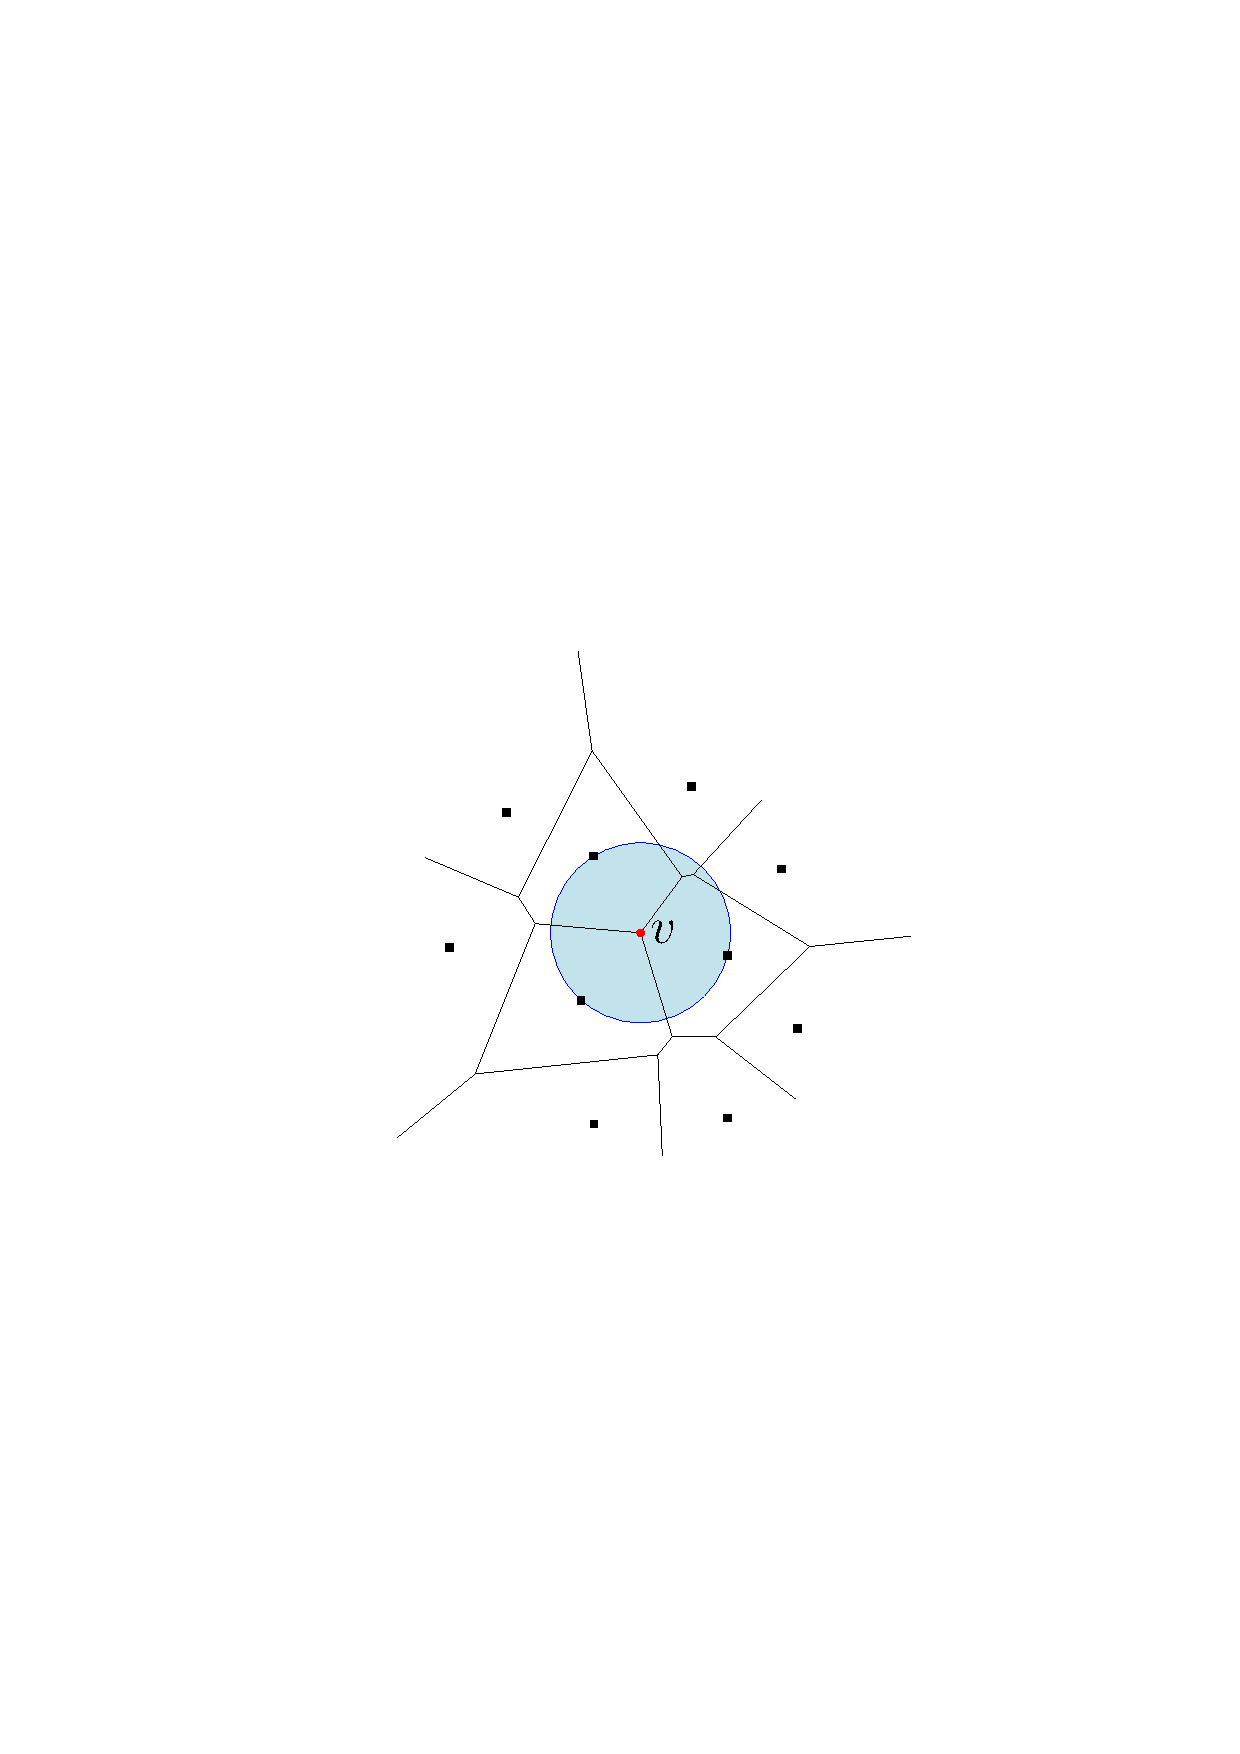
\includegraphics[width=4.9cm]{figs/voronoiCircle}
	\caption{Voronoi diagram, \\
		Voronoi vertex, circle}
	\label{fig:voronoiCircle}
\end{subfigure} ~~
\begin{subfigure}[b]{0.44\textwidth} \centering
	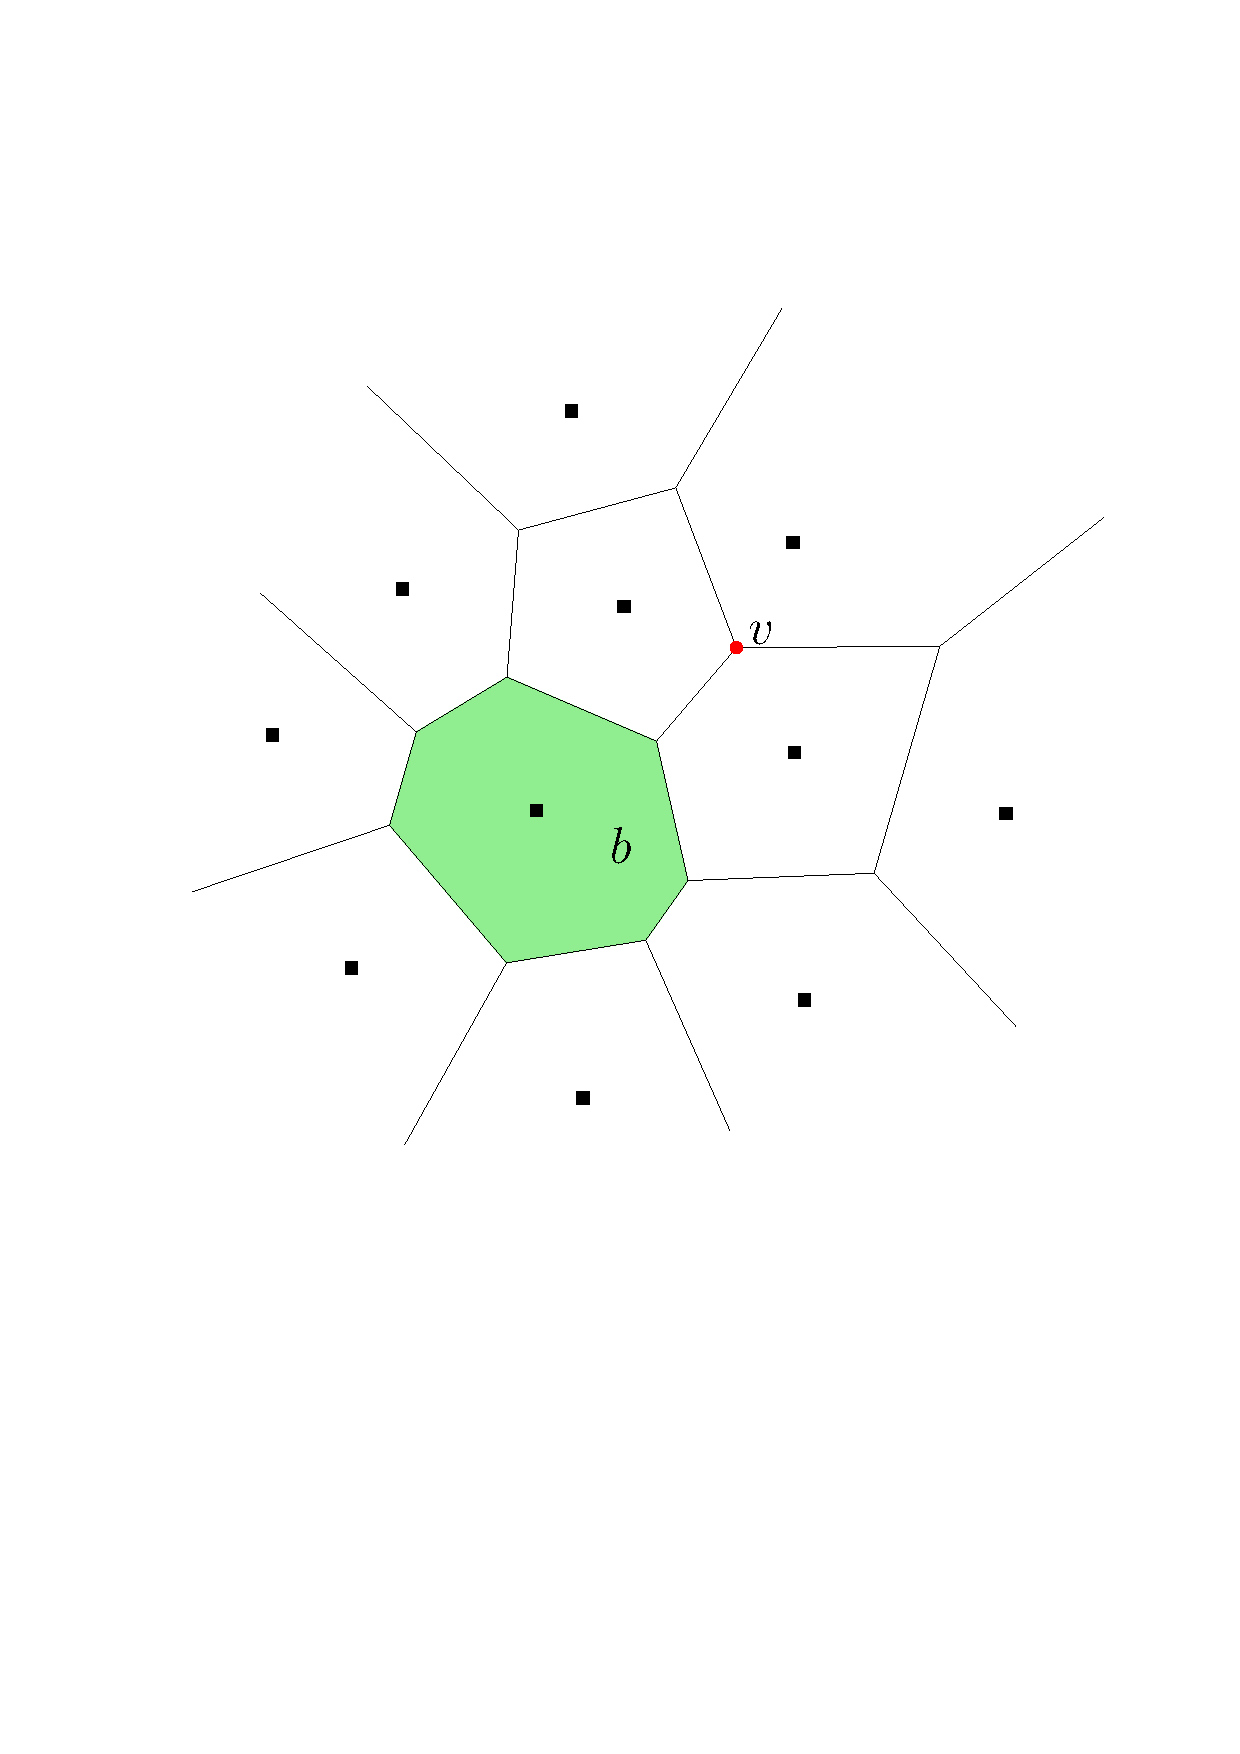
\includegraphics[width=4.7cm]{figs/neighbor.pdf}
	\caption{$v$ is a \paw of $b$ \\ \ }
	\label{fig:Paw}
\end{subfigure}
\end{figure} \end{frame}

\begin{frame} \frametitle{Dynamic VD setting}
When we are inserting new site $s_N$, the graph of the VD undergoes \\
operation called {\it flarb.} \vspace{-4mm}

\begin{figure}[h]
\centering
	\begin{subfigure}[t]{0.28\textwidth}
	\centering
	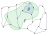
\includegraphics[width=3.8cm]{flarb/2flarb}
	\caption{Graph before flarb}
	\label{fig:flarb}
	\end{subfigure}
~
	\begin{subfigure}[t]{0.28\textwidth}
	\centering
	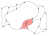
\includegraphics[width=3.8cm]{flarb/3afterflarb}
	\caption{Graph after flarb}
	\label{fig:afterflarb}
	\end{subfigure}
~
	\begin{subfigure}[t]{0.37\textwidth}
	\centering
	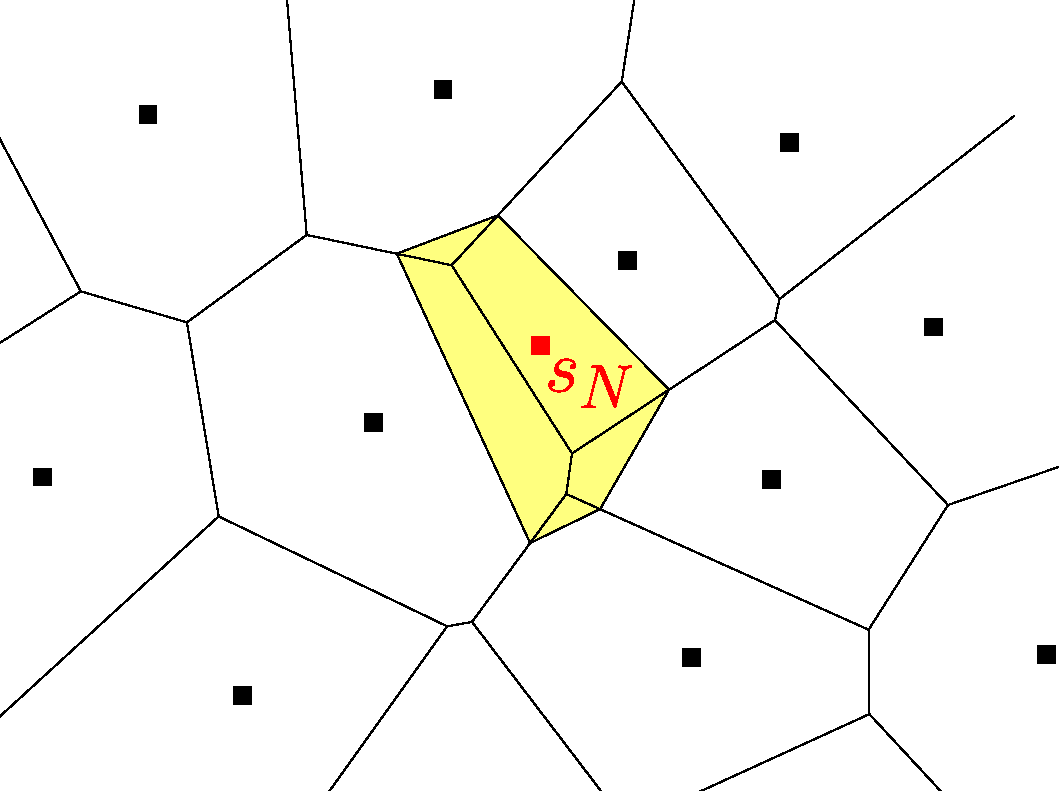
\includegraphics[width=4.4cm]{figs/identFlarb}
	\caption{Flarb on a VD}
	\label{fig:afterflarb}
	\end{subfigure}
\label{fig:exflarb}
\end{figure} \vspace{-2mm}

\begin{theorem}[\acite{incremental-vd}]
\label{thm:amorCost} \small
	The number of cells with combinatorial changes is $O(N^{\frac12})$ amortized, there are a constant number of combinatorial changes per cell, cells with changes are connected.
\end{theorem} \end{frame}

\begin{frame} \frametitle{Identifying changes}
\begin{tabular}{lcl}
\makecell[l]{
    \textcolor{hard}{\bf Theorem:} Let $g$ be a cell adjacent to $f$. \\
    Cell $g$ needs to undergo changes $\Longleftrightarrow$ \\
    circle of either of its vertices that are \\
    paws of $f$ encloses $s_N$.\qquad\acite{incremental-vd}
} & \qquad
& \makecell[c]{
	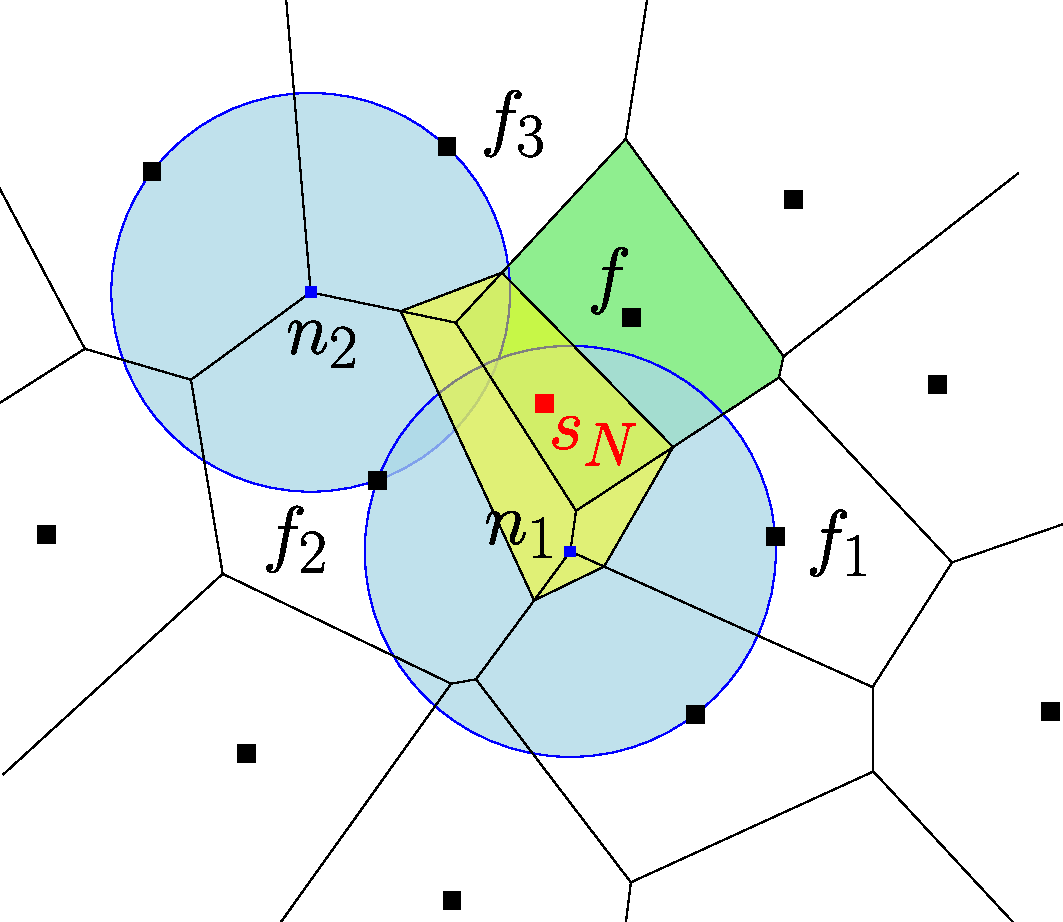
\includegraphics[width=5.4cm]{figs/identChanges}
} \end{tabular} \bigskip

\begin{block}{DCR structure (\acite{incremental-vd})}
	Returns all $k$ circles enclosing given point in $\Ot(k)$. Addition and deletion of \\
	a circle in $\Ot(1)$.
\end{block}
\end{frame}

\begin{frame} \frametitle{Big cells and small cells}
\vspace{2mm}
\begin{definition}
	A cell is \emph{big} if it has size at least $N^{\frac14}$. Otherwise it is \emph{small}.
\end{definition} \medskip

Small cells can be processed by brute force. For big cells we will need DCRs.
    \medskip

\begin{center}
	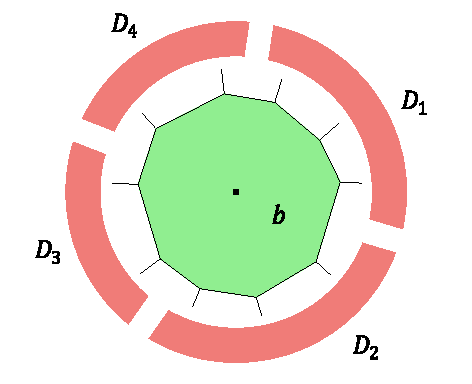
\includegraphics[width=5cm]{figs/consecDataStr}
\end{center}
\end{frame}